\section{Multiple Choice Questions (35 points) }

Just specify the correct answer.  No need to justify.

\subsection{Lasso (2 points)}

\question (True or False) Every L1-constrained regression problem is equivalent to some L1-regularized regression problem.

Recall that an L1-constrained regression problem is:
$$\argmin_{w,b} \sum_{(x,y)\in S} \left(y - (w^Tx + b)\right)^2,\ \ \ \      \mbox{s.t.}\ \ \ \ \ \|w\|_1 \leq C,
$$
and that an L1-regularized regression problem is:
$$\argmin_{w,b} \lambda\|w\|_1 + \sum_{(x,y)\in S} \left(y - (w^Tx + b)\right)^2.$$

\vspace{-0.2in}
\begin{solution}
True
\end{solution}

%\smallskip

\subsection{Bagging \& Bootstrap Sampling (3 points)}

\question
(Multiple Choice) Suppose we generate $M$ bootstraps $S'_1,\ldots,S'_M$ of a training set $S=\{(x_i,y_i)\}_{i=1}^N$.  For any specific $(x,y) \in S$, what is the probability that $(x,y)$ does not appear in ANY of $S'_1,\ldots,S'_M$?

(Recall that a bootstrap is a dataset with the same size as $S$ generated by sampling uniformly with replacement from $S$.)
%\smallskip

\textbf{Option A:}
$$
\left(1-\frac{1}{N}\right)^NM
$$
%\smallskip

\textbf{Option B:}
$$
\left(1-\frac{1}{N}\right)^{NM}
$$
%\smallskip

\textbf{Option C:}
$$
\left(1-\frac{1}{NM}\right)^{NM}
$$
%\smallskip

\textbf{Option D:}
$$
\left(1-\left(1-\frac{1}{NM}\right)^N\right)^M
$$
%\smallskip

\vspace{-0.2in}
\begin{solution}
B
\end{solution}

%\smallskip


\newpage

\subsection{Convolutional Filters (4 points)}


Consider the three convolutional filters below:

\begin{small}
\[K_{1} = \begin{bmatrix}
0.0043 & 0.0144 & 0.0214 & 0.0144 & 0.0043 \\
0.0144 & 0.0478 & 0.0712 & 0.0478 & 0.0144 \\
0.0214 & 0.0712 & 0.1062 & 0.0712 & 0.0214 \\
0.0144 & 0.0478 & 0.0712 & 0.0478 & 0.0144 \\
0.0043 & 0.0144 & 0.0214 & 0.0144 & 0.0043 
\end{bmatrix}\]

\[K_{2} = \begin{bmatrix}
0.0068 & 0.0225 & 0.0335 & 0.0225 & 0.0068 \\
0.0225 & 0.0746 & 0.1112 & 0.0746 & 0.0225 \\
0.0335 & 0.1112 & 0.1660 & 0.1112 & 0.0335 \\
0.0225 & 0.0746 & 0.1112 & 0.0746 & 0.0225 \\
0.0068 & 0.0225 & 0.0335 & 0.0225 & 0.0068 
\end{bmatrix}\]

\[K_{3} = \begin{bmatrix}
0 & 0 & 0 & 0 & 0\\
0 & 0 & 0 & 0 & 0\\
0 & 0 & 0.8 & 0 & 0\\
0 & 0 & 0 & 0 & 0\\
0 & 0 & 0 & 0 & 0
\end{bmatrix}\]
\end{small}

\question (Multiple Choice) If we apply $K_1$, $K_2$, and $K_3$ to Figure \ref{fig:convolve0}, which filter corresponds to which  image in Figure \ref{fig:convolve}?

\smallskip


\begin{figure}[h]
\vspace{-0.2in}
        \centering
	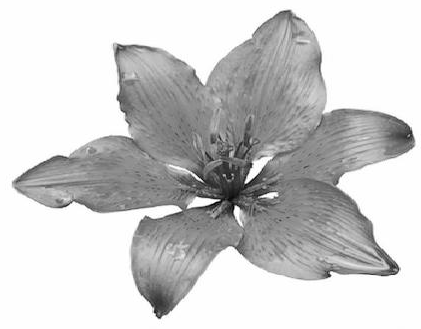
\includegraphics[scale=0.3]{image/white_black.png}
   \vspace{-0.1in}
   \caption{Original Image.  All pixel intensities are clipped between 0 and 1 (black=0 and white=1).}
\label{fig:convolve0}
   \end{figure}
   \begin{figure}[h]
\vspace{-0.2in}
   \centering
			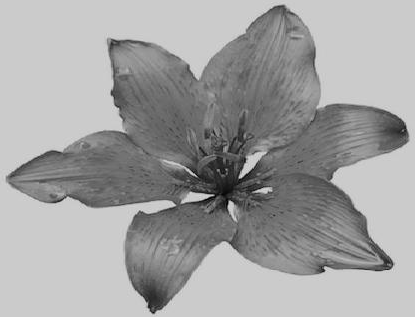
\includegraphics[scale=0.304]{image/darken.png}~~
			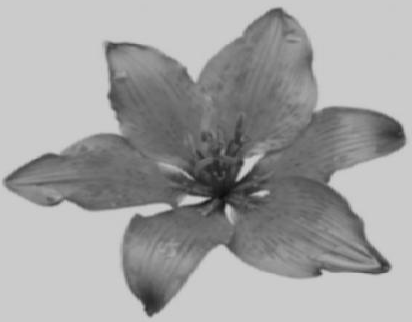
\includegraphics[scale=0.3]{image/dark_blur.png}~~
			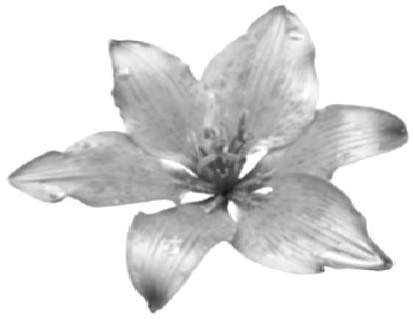
\includegraphics[scale=0.3]{image/brighten_blur.png}
   \vspace{-0.1in}
         \caption{Convolved Images (hint: the grey background is intentional)}
\label{fig:convolve}
\end{figure}

\vspace{-0.2in}
\begin{solution}
$K_1$ = Middle, $K_2$ = Right, $K_3$ = Left
\end{solution}


\smallskip





\subsection{Multiclass SVMs (3 points)}
\label{sec:multiclass_svm}


Consider the following 4-class multiclass SVM objective:
\begin{align*}
&\argmin_{w,\xi} \frac{1}{2}\|w\|^2 + \frac{C}{N}\sum_{i=1}^N \xi_i\\
\mbox{s.t.}\\
   & \forall i, \forall y' \in \{1,2,3,4\}:\ w_{y_i}^T x_i - w_{y'}^Tx_i \geq \textbf{1}_{[y_i\neq y']} - \xi_i
\end{align*}
where:
$$ w = \left[\begin{array}{c}
w_1\\
w_2\\
w_3\\
w_4
\end{array}\right],$$
and predictions are made via $\argmax_{y} w_y^Tx$.  In other words, each $\xi_i$ can be defined as:
\begin{eqnarray}
\xi_i = \max_{y' \in \{1,2,3,4\}} \left\{\textbf{1}_{[y_i\neq y']} - \left(w_{y_i}^T x_i - w_{y'}^Tx_i\right)\right\}\label{eqn:xi}.
\end{eqnarray}

Suppose for training data $(x_i,y_i)$ we have $y_i = 1$ and:
$$w_1^Tx_i  = 1.0,$$
$$w_2^Tx_i  = 1.5,$$
$$w_3^Tx_i  = 0.1,$$
$$w_4^Tx_i  = -0.8.$$

\smallskip

\question (Multiple Choice) Which $\yh\in\{1,2,3,4\}$  is the maximizer of \eqref{eqn:xi}?


\begin{solution}
$\yh = 2$
\end{solution}

\smallskip

\subsection{Feature Maps (3 points)}

Consider the following 3-class multiclass feature map:
\begin{eqnarray}
\phi(x,y) = \left[\begin{array}{c}
\textbf{1}_{[y=1]} x\\
\textbf{1}_{[y=2]} x\\
\textbf{1}_{[y=3]} x\\
-\textbf{1}_{[y\in\{1,2\}]} x
\end{array}\right],
   \label{eqn:feature}
   \end{eqnarray}
where predictions are made via $\argmax_{y\in\{1,2,3\}} w^T\phi(x,y)$.

\question (Multiple Choice) What is the effect of using \eqref{eqn:feature} versus a ``conventional'' multiclass feature map of:
\begin{eqnarray}
\phi(x,y) = \left[\begin{array}{c}
\textbf{1}_{[y=1]} x\\
\textbf{1}_{[y=2]} x\\
\textbf{1}_{[y=3]} x\\
\end{array}\right].
   \label{eqn:feature2}
   \end{eqnarray}

\textbf{Option A:} Compared to \eqref{eqn:feature2}, in \eqref{eqn:feature} the model scores for Class 1 \& 2 are encouraged to be correlated.
\smallskip

\textbf{Option B:} Compared to \eqref{eqn:feature2}, in \eqref{eqn:feature} the model scores for Class 1 \& 2 are encouraged to be anti-correlated.
\smallskip

\textbf{Option C:} Either A or B are possible depending on the specific training data.
\smallskip

(Recall that the model score for a class $y'$ is just $w^T\phi(x,y')$.)

\begin{solution}
A
\end{solution}

\smallskip

\subsection{Hard-Margin SVMs (5 points)}

A hard margin SVM can be written as:
%\begin{align*}
%& \argmin_{w,b} \frac{1}{2}\|w\|^2\\
%\mbox{s.t.}\\
%& \forall (x,y)\in S: y(w^T x -b) \geq 1
%\end{align*}
\begin{figure}[h]
\vspace{-0.12in}
\centering
%\includegraphics[scale=0.3]{image/svm.pdf}
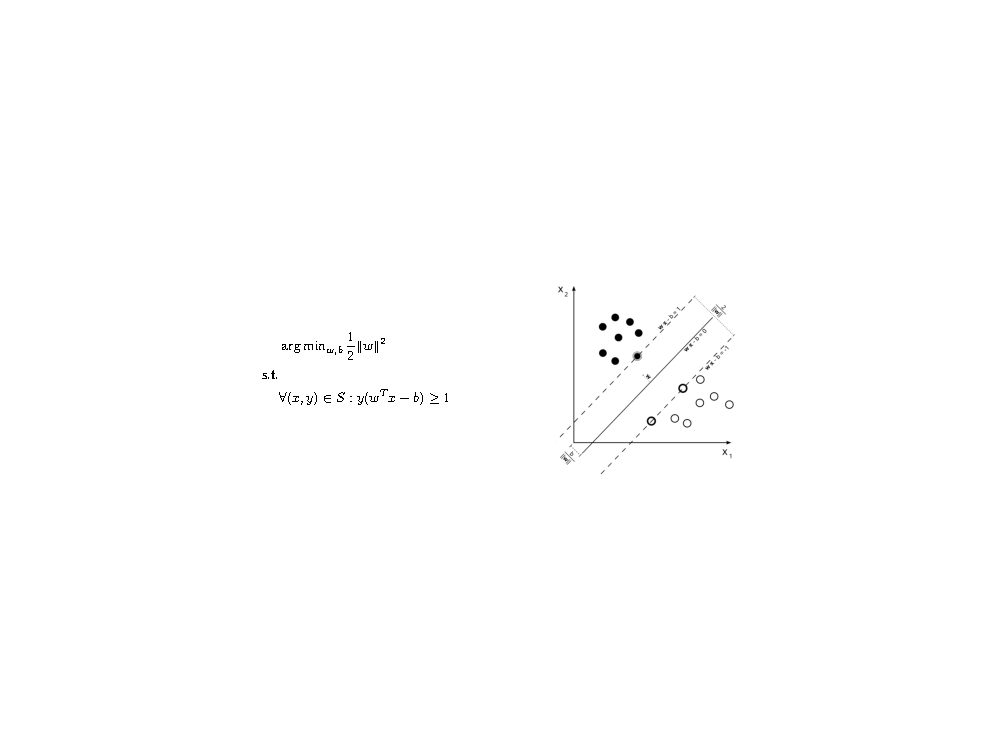
\includegraphics[scale=1.65]{image/svm2.pdf}
\vspace{-0.1in}
\end{figure}

The figure to the right depicts a visualization of the hard-margin SVM for a 2-dimensional example (image source Wikipedia).  The data points that are on the margin (for which the inequality constraint in the training optimization problem is a tight equality) are known as ``support vectors''.


\question (True or False) If the data is not linearly separable, then a hard-margin SVM returns $w=0$.  

\begin{solution}
False
\end{solution}


\smallskip 



\question (Multiple Choice) Assume the data is linearly separable. What happens when we remove a data point that is NOT a support vector from the training set, and then retrain the model?

\smallskip

\textbf{Option A:} The solution $w$ and $b$ do not change from before.
\smallskip

\textbf{Option B:} The solution changes, and the training error is reduced.
\smallskip

\textbf{Option C:} The solution changes, and the training error is increased.
\smallskip

\vspace{-0.1in}
\begin{solution}
A
\end{solution}

\subsection{AdaBoost (2 points)}
\question (True or False)  Each iteration of AdaBoost is guaranteed to reduce the training 0/1 Loss of the aggregate model. 

Recall that the aggregate model of AdaBoost at iteration $T$ is:
$$f_T(x) = \sum_{t=1}^T \alpha_t h_t(x)\in\Re,$$
and predictions are made via the sign of $f_T(x)$: $h_T(x) = \texttt{sign}(f_T(x))$.  %Also recall that the Exponential Loss of a data point $(x,y)$ with $y \in \{-1,+1\}$ is
%$$L(y,f_T(x)) = \exp\left\{-yf_T(x)\right\}.$$


\vspace{-0.1in}
\begin{solution}
False
\end{solution}

\smallskip

\subsection{Tensor Model Training (2 points)}

\question (True or False) Every L2-regularized tensor latent-factor regression problem can be optimized via alternating closed-form optimization (i.e., converges to a local optimum).

Recall that a L2-regularized tensor regression problem can be written as:
$$\argmin_{U,V,W} \frac{1}{2}\left(\|U\|_F^2 + \|V\|_F^2 + \|W\|_F^2\right) + \frac{1}{2}\sum_{(a,b,c)\in S}\left(Y_{a,b,c} - \langle u_a,v_b,w_c\rangle\right)^2,$$
where  $u_a$, $v_b$, and $w_c$ correspond to the $a$-th column of $U$, the $b$-th column of $V$, and the $c$-th column of $W$, respectively.  The three-way dot product is defined as:
$$\langle u_a,v_b,w_c\rangle = \sum_{k=1}^K u_{a,k}v_{b,k}, w_{c,k}.$$
Alternating closed-form optimization implies that $U$ (likewise $V$ or $W$) can be solved optimally in closed-form if one holds the other two matrices $V$ and $W$ fixed.


\vspace{-0.1in}
\begin{solution}
True
\end{solution}

\smallskip

\subsection{Bias-Variance Decomposition (2 points)}

Let $f_S \in F_S$ denote a set of linear regression models  trained on training set $S$ using different learning algorithms (e.g., each $f_S$ is  trained using a different regularization strength).
Let $\fh_S$ denote the $f_S \in F_S$ that has the lowest bias  in the bias-variance decomposition.

\question (True or False)  The minimum bias learning algorithm is guaranteed to have the smallest test squared loss.  In other words, the test error of $\fh_S$ is guaranteed to be lower than the test error of any other $f_S$:
$$\forall f_S \in F_S:\ E_{(x,y)\sim P(x,y)} E_{S}\left[\left(y-\fh_S(x)\right)^2\right] \leq E_{(x,y)\sim P(x,y)} E_{S}\left[(y-f_S(x))^2\right],$$
where $P(x,y)$ denotes the test distribution.

\begin{solution}
False
\end{solution}

\smallskip

\subsection{HMM EM Learning (3 points)}

\question
(Multiple Choice)
During EM training in the unsupservised setting, what best describes what happens when you initialize $P(y^j|y^{j-1})$ and $P(x^j|y^j)$ to both be the uniform distribution?

\smallskip

\textbf{Option A:}  Nothing special, you just converge to some local optimum.
\smallskip

\textbf{Option B:}  You converge to a degenerate local optimum where all the hidden states learn the same thing.
\smallskip

\textbf{Option C:}  You get a divide-by-0 error and training crashes.
\smallskip

Recall that an HMM model is specified by:
$$P(x,y) = P(End|y^M)\prod_{j=1}^M P(x^j|y^j)P(y^j|y^{j-1}),$$
the unsupervised learning problem is specified by
$$\argmax_{\Theta} \prod_{x\in S} P(x) = \argmax_{\Theta} \prod_{x\in S} \sum_{y'} P(x,y'),$$
where $S$ denotes the training set and $\Theta$ denotes all the HMM model parameters. 
The EM algorithm alternates between inferring the distribution of sequences $y'$ for each training example $x$ and using that inferred distribution to estimate better model parameters $\Theta$.  


\begin{solution}
B
\end{solution}



\subsection{Non-Negative Matrix Factorization (2 points)}

Consider the matrix factorization problem of minimizing squared reconstruction error:
$$\argmin_{U\in \Re^{N\times K}, V\in \Re^{M\times K}} \|Y - UV^T\|_{Fro}^2,$$
where $Y \in \Re^{N \times M}$ is the matrix we wish to encode in a low-rank model, and $U$ and $V$ are our model components.

\question (True or False) Suppose $Y$ is non-negative.  If we enforce $U$ and $V$ to also be non-negative, then we typically need a larger latent dimension $K$ to achieve the same squared reconstruction error compared to allowing $U$ and $V$ to take negative values.

\begin{solution}
True
\end{solution}

\subsection{Decision Trees (2 points)}

\question (True or False) Given infinite training data (sampled i.i.d. from the test distribution), decision trees can essentially learn arbitrary classifier functions. (Ignore the distinction between countably vs uncountably infinite, this is a high-level conceptual question.)

\begin{solution}
True
\end{solution}

\subsection{Overfitting (2 points)}
\question (True or False) Given infinite training data (sampled i.i.d. from the test distribution), it is essentially impossible to overfit. (Ignore the distinction between countably vs uncountably infinite, this is a high-level conceptual question.)

\begin{solution}
True
\end{solution}
